\documentclass[]{article}

\usepackage[utf8]{inputenc}
\usepackage{url}
\usepackage{float}
\usepackage{breakurl} 
\usepackage[breaklinks]{hyperref}
\usepackage{lipsum}
\usepackage{multicol}
\usepackage{graphicx}
\usepackage{float}
\usepackage{psfrag}
\usepackage{amssymb}
\usepackage{graphics}
\usepackage{amsmath}
\usepackage{url}
\usepackage{algorithm}
\usepackage{algpseudocode}
\usepackage{tabularx}
\usepackage{filecontents}
\usepackage{url}
\usepackage{multirow}
\usepackage{mathtools}
\usepackage{scrextend}
\usepackage[flushleft]{threeparttable}
\usepackage{subfigure}
\usepackage{textcomp}
\usepackage{tablefootnote}
\usepackage{graphicx}


\def\UrlBreaks{\do\/\do-}

\algblockdefx[Foreach]{Foreach}{EndForeach}[1]{\textbf{foreach} #1 \textbf{do}}{\textbf{end foreach}}

\providecommand{\algorithminput}[1]{
	~\\
	\textbf{Input:}\\
	\begin{tabularx}{\textwidth}{rl}#1\end{tabularx}
}
\providecommand{\algorithmoutput}[1]{
	~\\
	\textbf{Output:}\\
	\begin{tabularx}{\textwidth}{rl}#1\end{tabularx}
}

\newcommand{\Break}{\textbf{break}}


%opening
\title{\textit{Undersampling} Representativo de Classe Dominante por Fator de Qualidade Baseado em Multiplicadores de Lagrange  }
\author{Paulo Cirino}

\begin{document}
	
	\maketitle
	
	\begin{abstract}
		
	\end{abstract}
	
	\section{Introdução}
	
	Esse trabalho é fundamento em um algorítimo de \textit{fuzzy clustering}, à ser publicado, que foi criado para acelerar o método \textit{Fuzzy C Means}. No trabalho feito, se atinge o objetivo por meio da remoção de pontos da bordas com o auxilio de um fator de qualidade, que diz respeito a pertinência de cada amostra à todos os \textit{clusters}.
	
	Os algorítimo de  \textit{fuzzy clustering } permitem que uma amostra de um \textit{data set} pertença, ao mesmo tempo, à múltiplos agrupamentos. O nível que uma amostra pertence a cada \textit{cluster} é tradicionalmente chamado de \textbf{pertinência $\mu_{i}(x_j)$}, que é a pertinência da amostra $x_j$ para o \textit{cluster} $i$.
	
	A função de custo $J$, associada à problemas de \textit{fuzzy clustering}, pode ser definida em 
	\ref{eqJ1}.
	\begin{equation}
	\label{eqJ1}
	\begin{aligned}
	& {\text{min}}
	& & J \\
	& \text{sujeito a}
	& & \sum_{k=1}^c u_{ik}=1,   \quad k=1,2,...,N \\
	\end{aligned}
	\end{equation}
	
	Onde $J$ é definido em \ref{eqJ2}.
	\begin{equation}
	\label{eqJ2}
	J = \sum_{i=1}^c \sum_{k=1}^N u_{ik}^2 d_{ik}^2
	\end{equation} 
	
	Nessa situação $\mu_{ik}$, é a pertinência da amostra $k$ em relação ao centro $i$. Adotando a solução de Multiplicadores de Lagrange, a nova função de custo assume a forma descrita em \ref{eqJ22}, com derivadas parciais \ref{eqdjdl} e \ref{eqdjdu}. 
	
	\begin{equation}
	\label{eqJ22}
	J = \sum_{i=1}^c \sum_{k=1}^N \left [  u_{ik}^2 d_{ik}^2 - \lambda (\sum_{m=1}^c u_{mk}-1)\right]
	\end{equation}
	
	\begin{equation}
	\label{eqdjdl}
	{{\partial J} \over {\partial \lambda}} = \sum_{m=1}^c u_{mk}-1 : {{\partial J} \over {\partial \lambda}} = 0 \implies \sum_{i=1}^c u_{ik}=1
	\end{equation}
	
	\begin{equation}
	\label{eqdjdu}
	{{\partial J} \over {\partial u_{st}}} = 2u_{st} d_{st}^2 - \lambda : {{\partial J} \over {\partial u_{st}}} = 0 \implies u_{st} = {\lambda \over {2d_{st}^2}}
	\end{equation}
	
	Assim, a equação \ref{eqLamdaT}, representa cada um dos multiplicadores de Lagrange do \textit{data set}.
	
	\begin{equation}
	\label{eqLamdaT}
	\lambda_{k} = {2 \over {\sum_{j=1}^c {1 \over d_{jk}^2}}}, \quad k=1,2...,N
	\end{equation}
	
	Assim é possível definir uma medida de qualidade para cada amostra, descrita na equação, \ref{eqqk}. A medida $q_k$ de qualidade, é obtida para cada amostra $\mathbf{x}_k$ de $\mathbf{X}=\{x_i \in \mathbb{R^d} | i=1...N\}$, e representa uma medida de incerteza da pertinência $\mu_{ik}$.
	
	\begin{equation}
	\label{eqqk}
	q_k = c^c \prod_{i=1}^c {1 \over \mu_{ik}}
	\end{equation}
	
	Substituindo a equação \ref{eqdjdu} em \ref{eqqk}, podemos representar $q_k$ em \ref{eqqk_lambda_a0}
	
	\begin{equation}
	\label{eqqk_lambda_a0}
	q_k = {2 \over {\lambda_k}} c^c \prod_{i=1}^c d_{ik}^2
	\end{equation}
	
	É importante notar que amostras fortemente ligadas a um determinado centro, terão $q_k$ muito próximo à $0$, aquelas que estão distantes terão valores tendendo à $\infty$.
	
	Uma forma alternativa de enxergar o índice de qualidade é substituindo a equação \ref{eqLamdaT} em \ref{eqqk_lambda_a0}.
	
	\begin{equation}
	\label{qk_final}
	q_k = c^c  \frac{ \prod_{i=1}^c d_{ik}^2} {\sum_{i = 1}^{c}d_{ik}^2}
	\end{equation}
	
	Uma forma de visualizar essa qualidade é por meio do gráfico abaixo:
	
	\begin{figure}[H]
		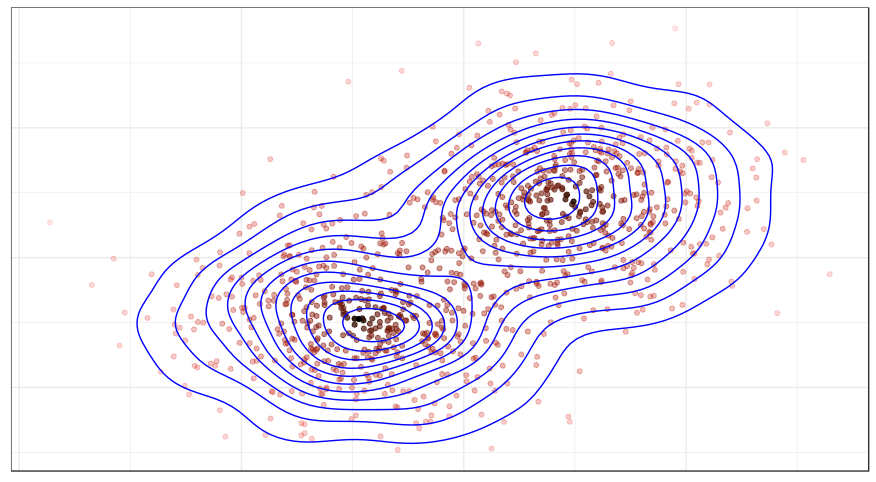
\includegraphics[width=\linewidth]{imgs/qualidade_plot.png}
		\caption{Gráfico de 2 normais, onde cor e as curvas de nível representam a qualidade}
		\label{fig:qplot}
	\end{figure}
	
	Visto que, é possível calcular um índice de qualidade para cada amostra que diz respeito à quanto um ponto faz parte ou não de um agrupamento. É possível utilizar a informação da qualidade para fazer seleção de amostras pertinentes.
	
	Em um senário de classificação desbalanceada, é possível então, fazer uma subamostragem da classe dominante, no sentido de balancear o problema. 
	
	\section{Método}
	Foram propostos um total de 5 abordagens de amostragem utilizando essa qualidade. Para esse método, foram considerados apenas problemas binários desbalanceados. 
	
	O que é comum em todas as abordagens é que foram selecionadas $N_{minority}$ das $N_{majority}$ amostras da classe majoritária, tal que $N_{minority} < N_{majority}$.
	
	\subsection{briSelect} 
	
	A primeira abordagem proposta foi a de \textit{briSelection}, onde são selecionadas as $N_{minority}$ amostras da classe majoritária com maior fator de qualidade. 
	
	Essa abordagem têm o efeito de selecionar os pontos marginais da classe dominante. Isso pode ser positivo no sentido de amostras apenas os pontos que definem o contorno da superfície de decisão, porém, pode ser muito negativo em situações onde os dados possuem muitos \textit{outliers}. 
	
	\subsection{briSelect++} 
	s abordagem \textit{briSelect++} é inspiradas na metodologia de inicialização do método \textbf{FCM++}.
	
	Isso é feito de forma que quanto maior a qualidade de uma amostra da classe dominantes, maior a probabilidade de essa amostra ser selecionada, assim como mostra a equação \ref{briSelectionPlusPlusEq}.
	
	\begin{equation}
	\label{briSelectionPlusPlusEq}
	P(x_k\mid q_k) = N_{minority} \frac{q_k}{\sum_{k = 1}^{N_{majority}} q_k}  \quad k = 1,2,...,N_{majority}
	\end{equation}
	
	Essa metodologia possui a vantagem de amostrar a distribuição da classe dominante como um todo, nas regiões centrais por conta da alta densidade de pontos e nas periferias por causa do alto índice de qualidade. Isso possui uma vantagem de representar todos os dados e não só as bordas.
	
	\subsection{briSelect$--$} 
	A metodologia \textit{briSelection$--$} é exatamente igual ao \textit{$briSelect++$}, só que $q_k$ é substituído por $\frac{1}{q_k}$, como mostra a formula \ref{briSelectionNegNegEq}.
	
		\begin{equation}
		\label{briSelectionNegNegEq}
		P(x_k\mid q_k) = N_{minority} \frac{\frac{1}{q_k}}{\sum_{k = 1}^{N_{majority}} \frac{1}{q_k}}  \quad k = 1,2,...,N_{majority}
		\end{equation}
		
	Essa alteração na formulação permite que o centro da distribuição da classe dominante seja muito bem representado, mas ainda criando uma probabilidade de os pontos da margem também serem amostrados.
	
	\subsection{briSelectionLog++ e briSelectionLog$--$} 
	Quando observamos a distribuição do fator de qualidade, percebemos que ela não é normal mas sim uma log-normal.
	
	\begin{figure}[H]
		\centering
		\begin{minipage}[b]{0.4\textwidth}
			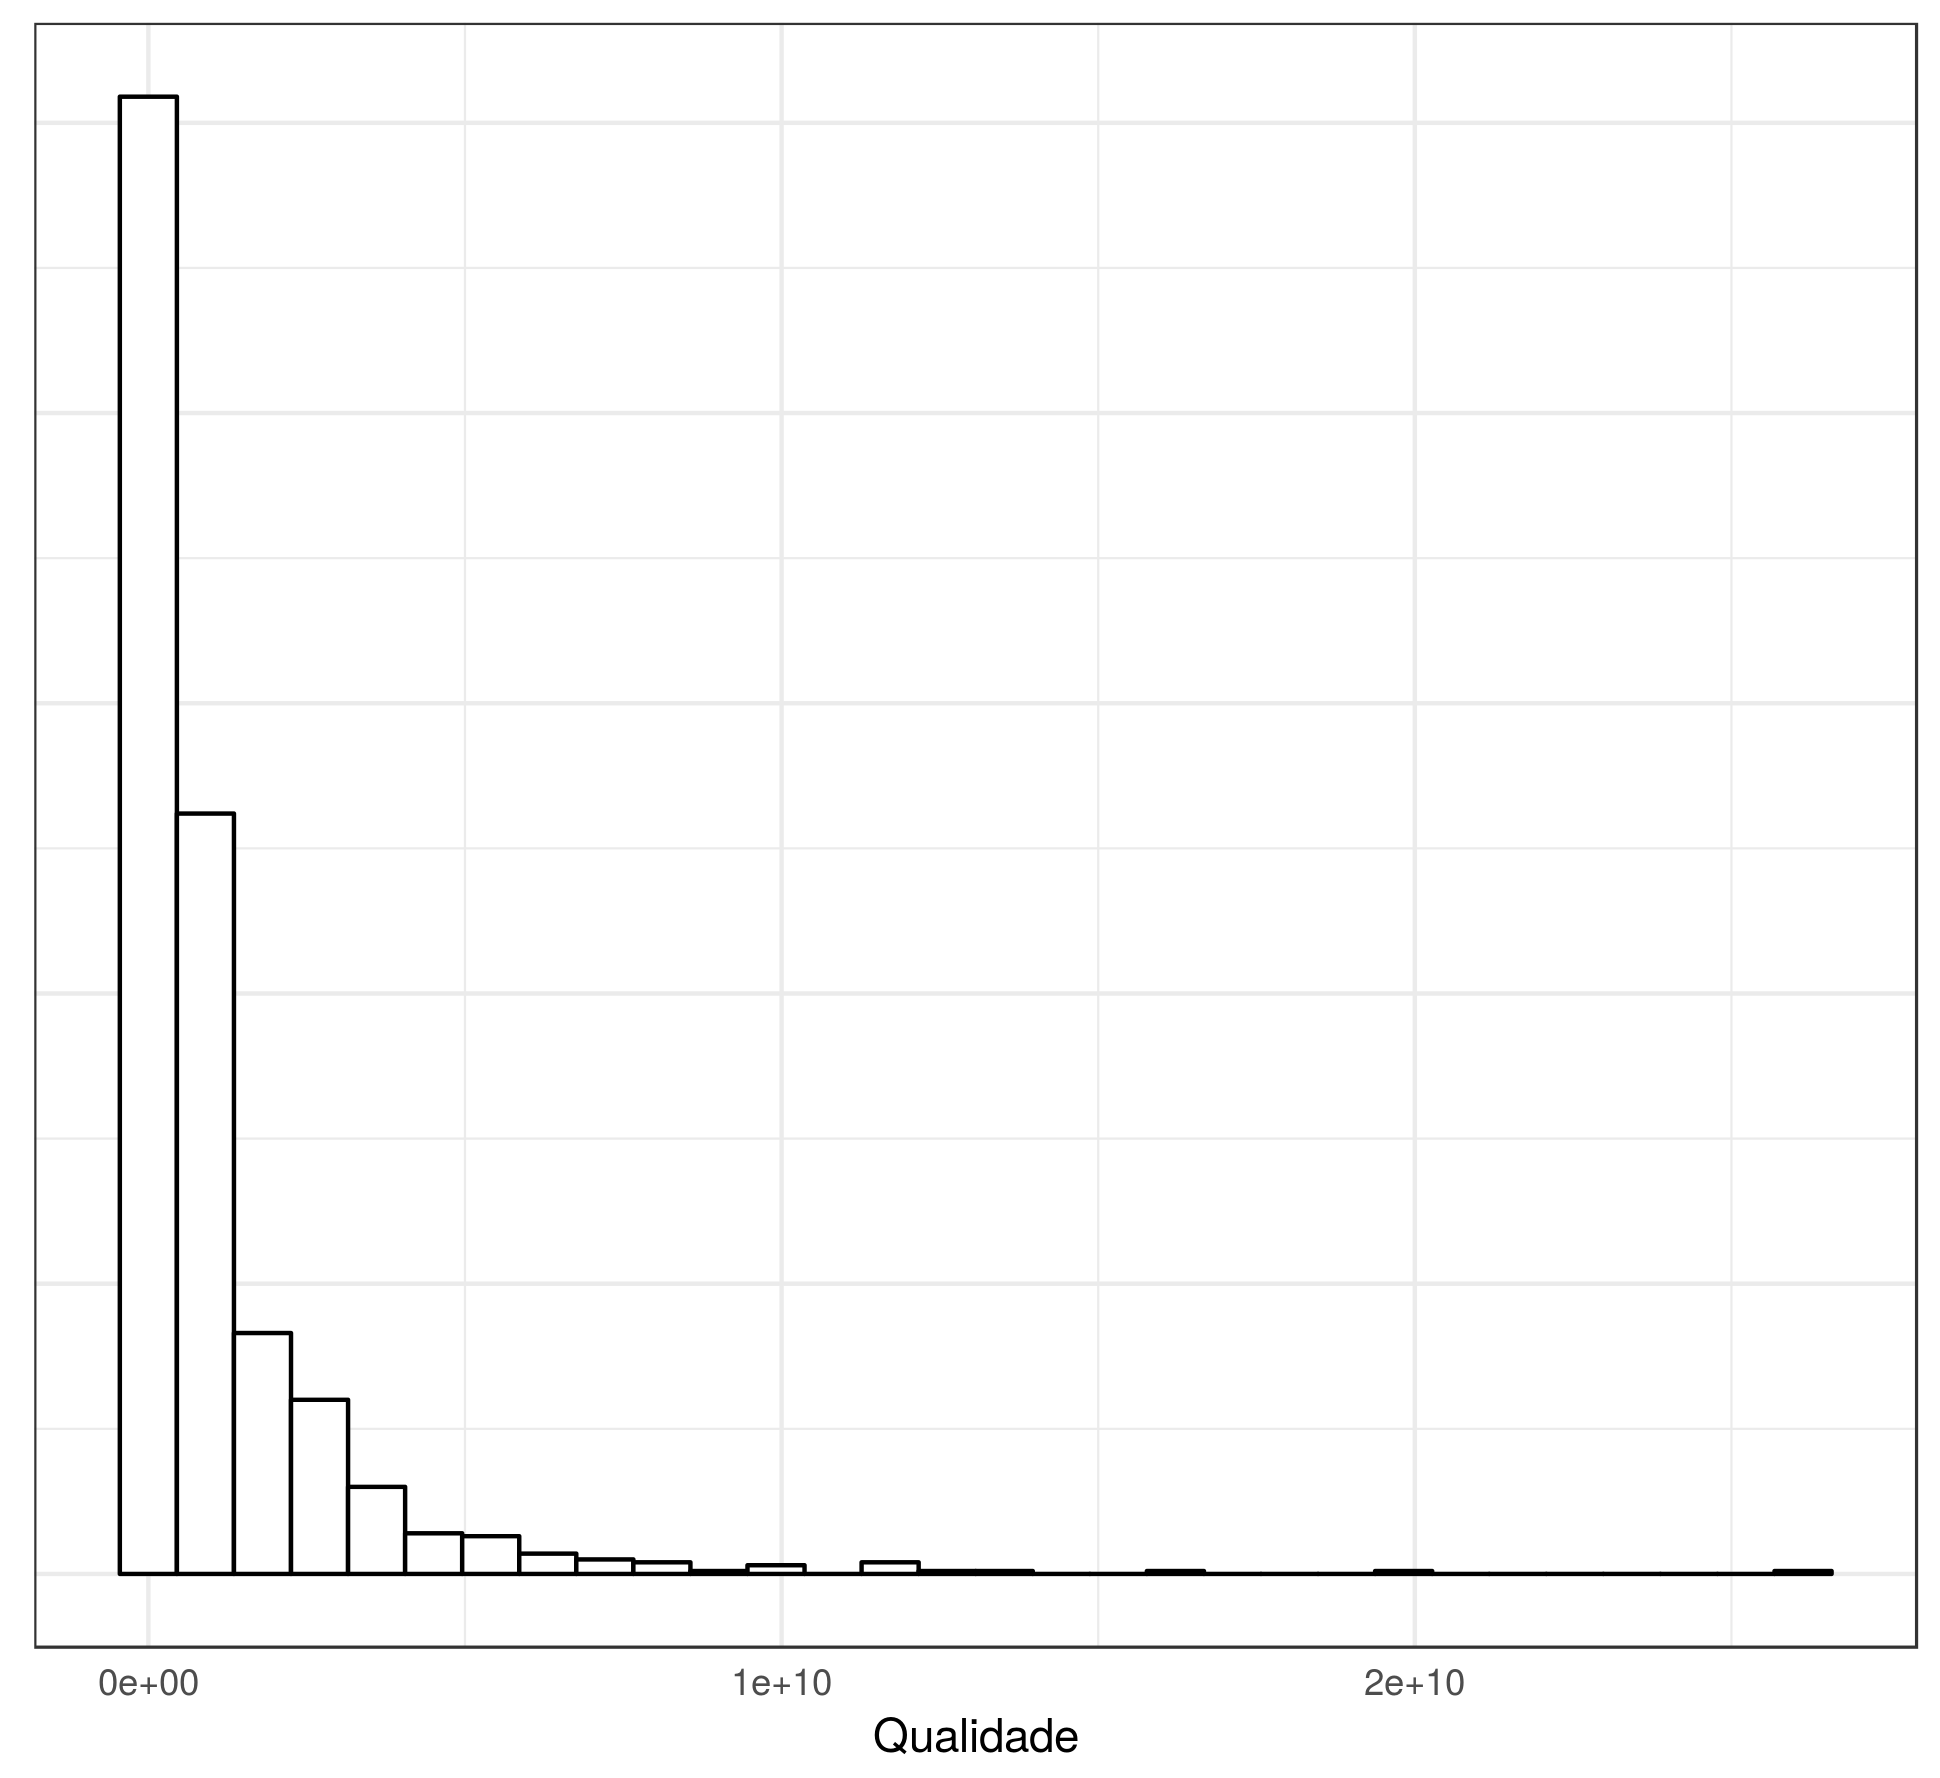
\includegraphics[width=\textwidth]{imgs/histograma.png}
			\caption{Histograma da Qualidade}
		\end{minipage}
		\hfill
		\begin{minipage}[b]{0.4\textwidth}
			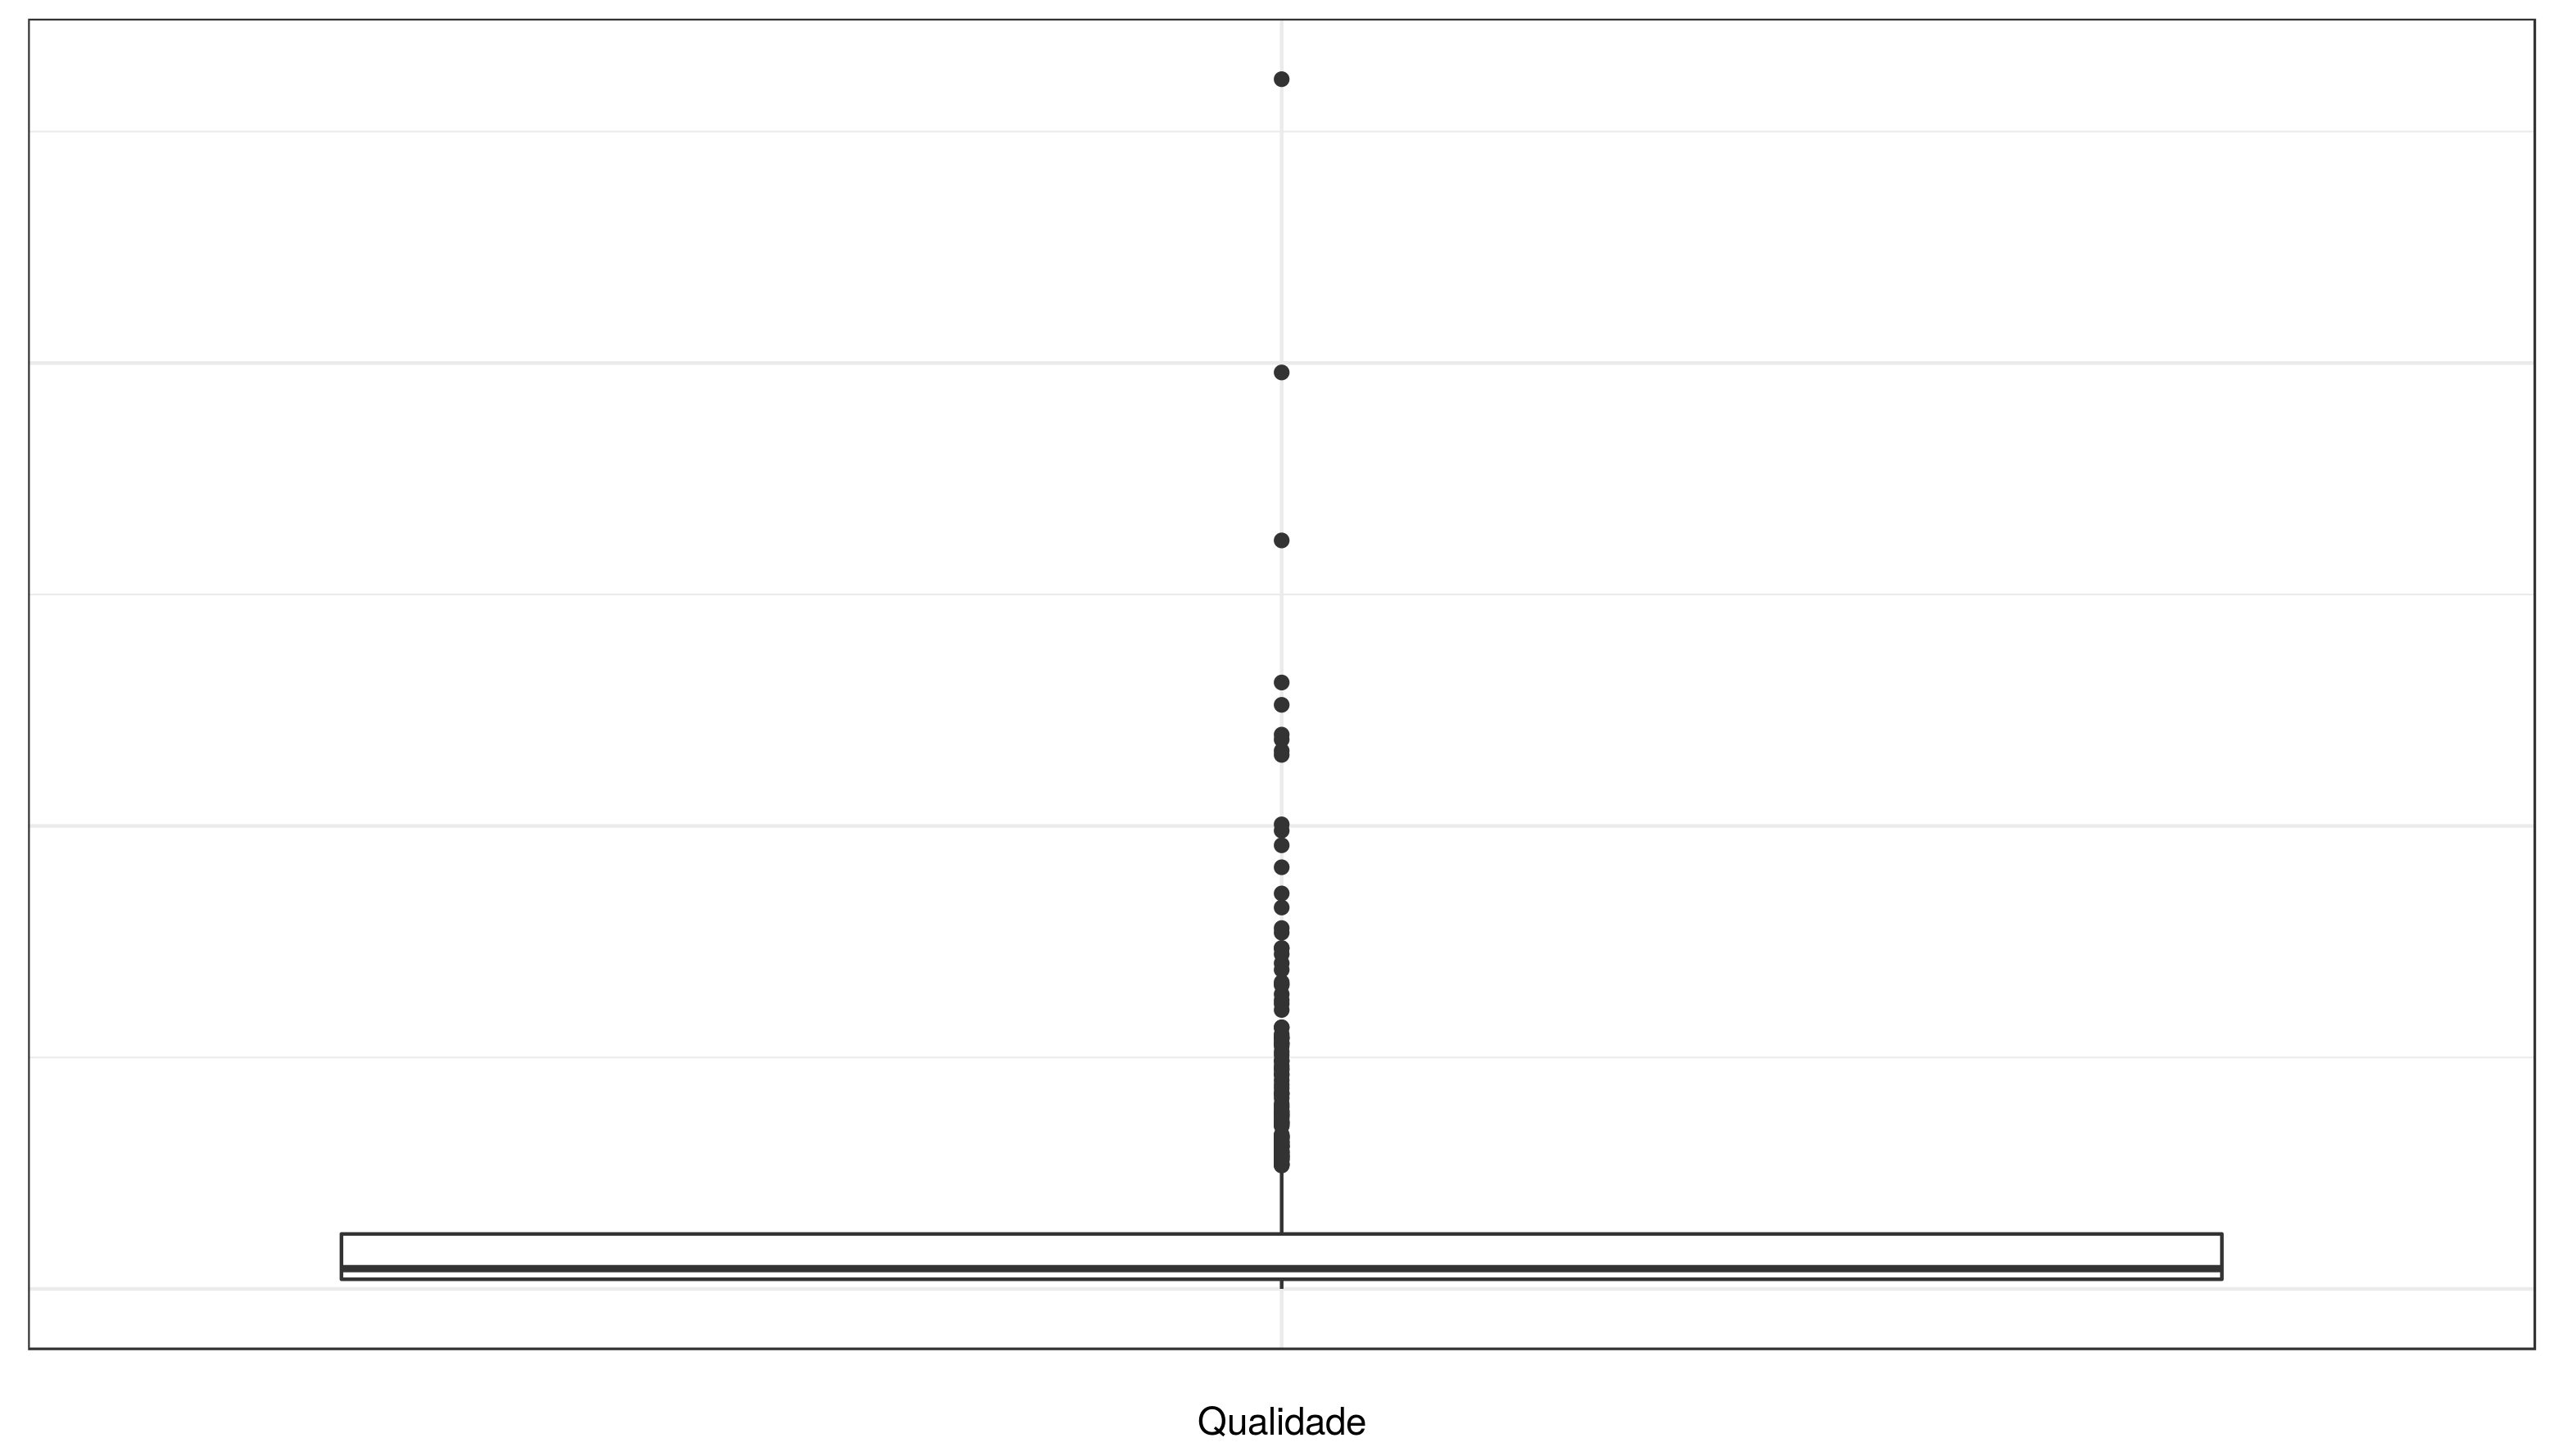
\includegraphics[width=\textwidth]{imgs/boxplot.png}
			\caption{Boxplot da Qualidade}
		\end{minipage}
	\end{figure}
	
	Mas é possível fazer uma normalização dessa qualidade por meio do logaritmo.
	
		\begin{figure}[H]
			\centering
			\begin{minipage}[b]{0.4\textwidth}
				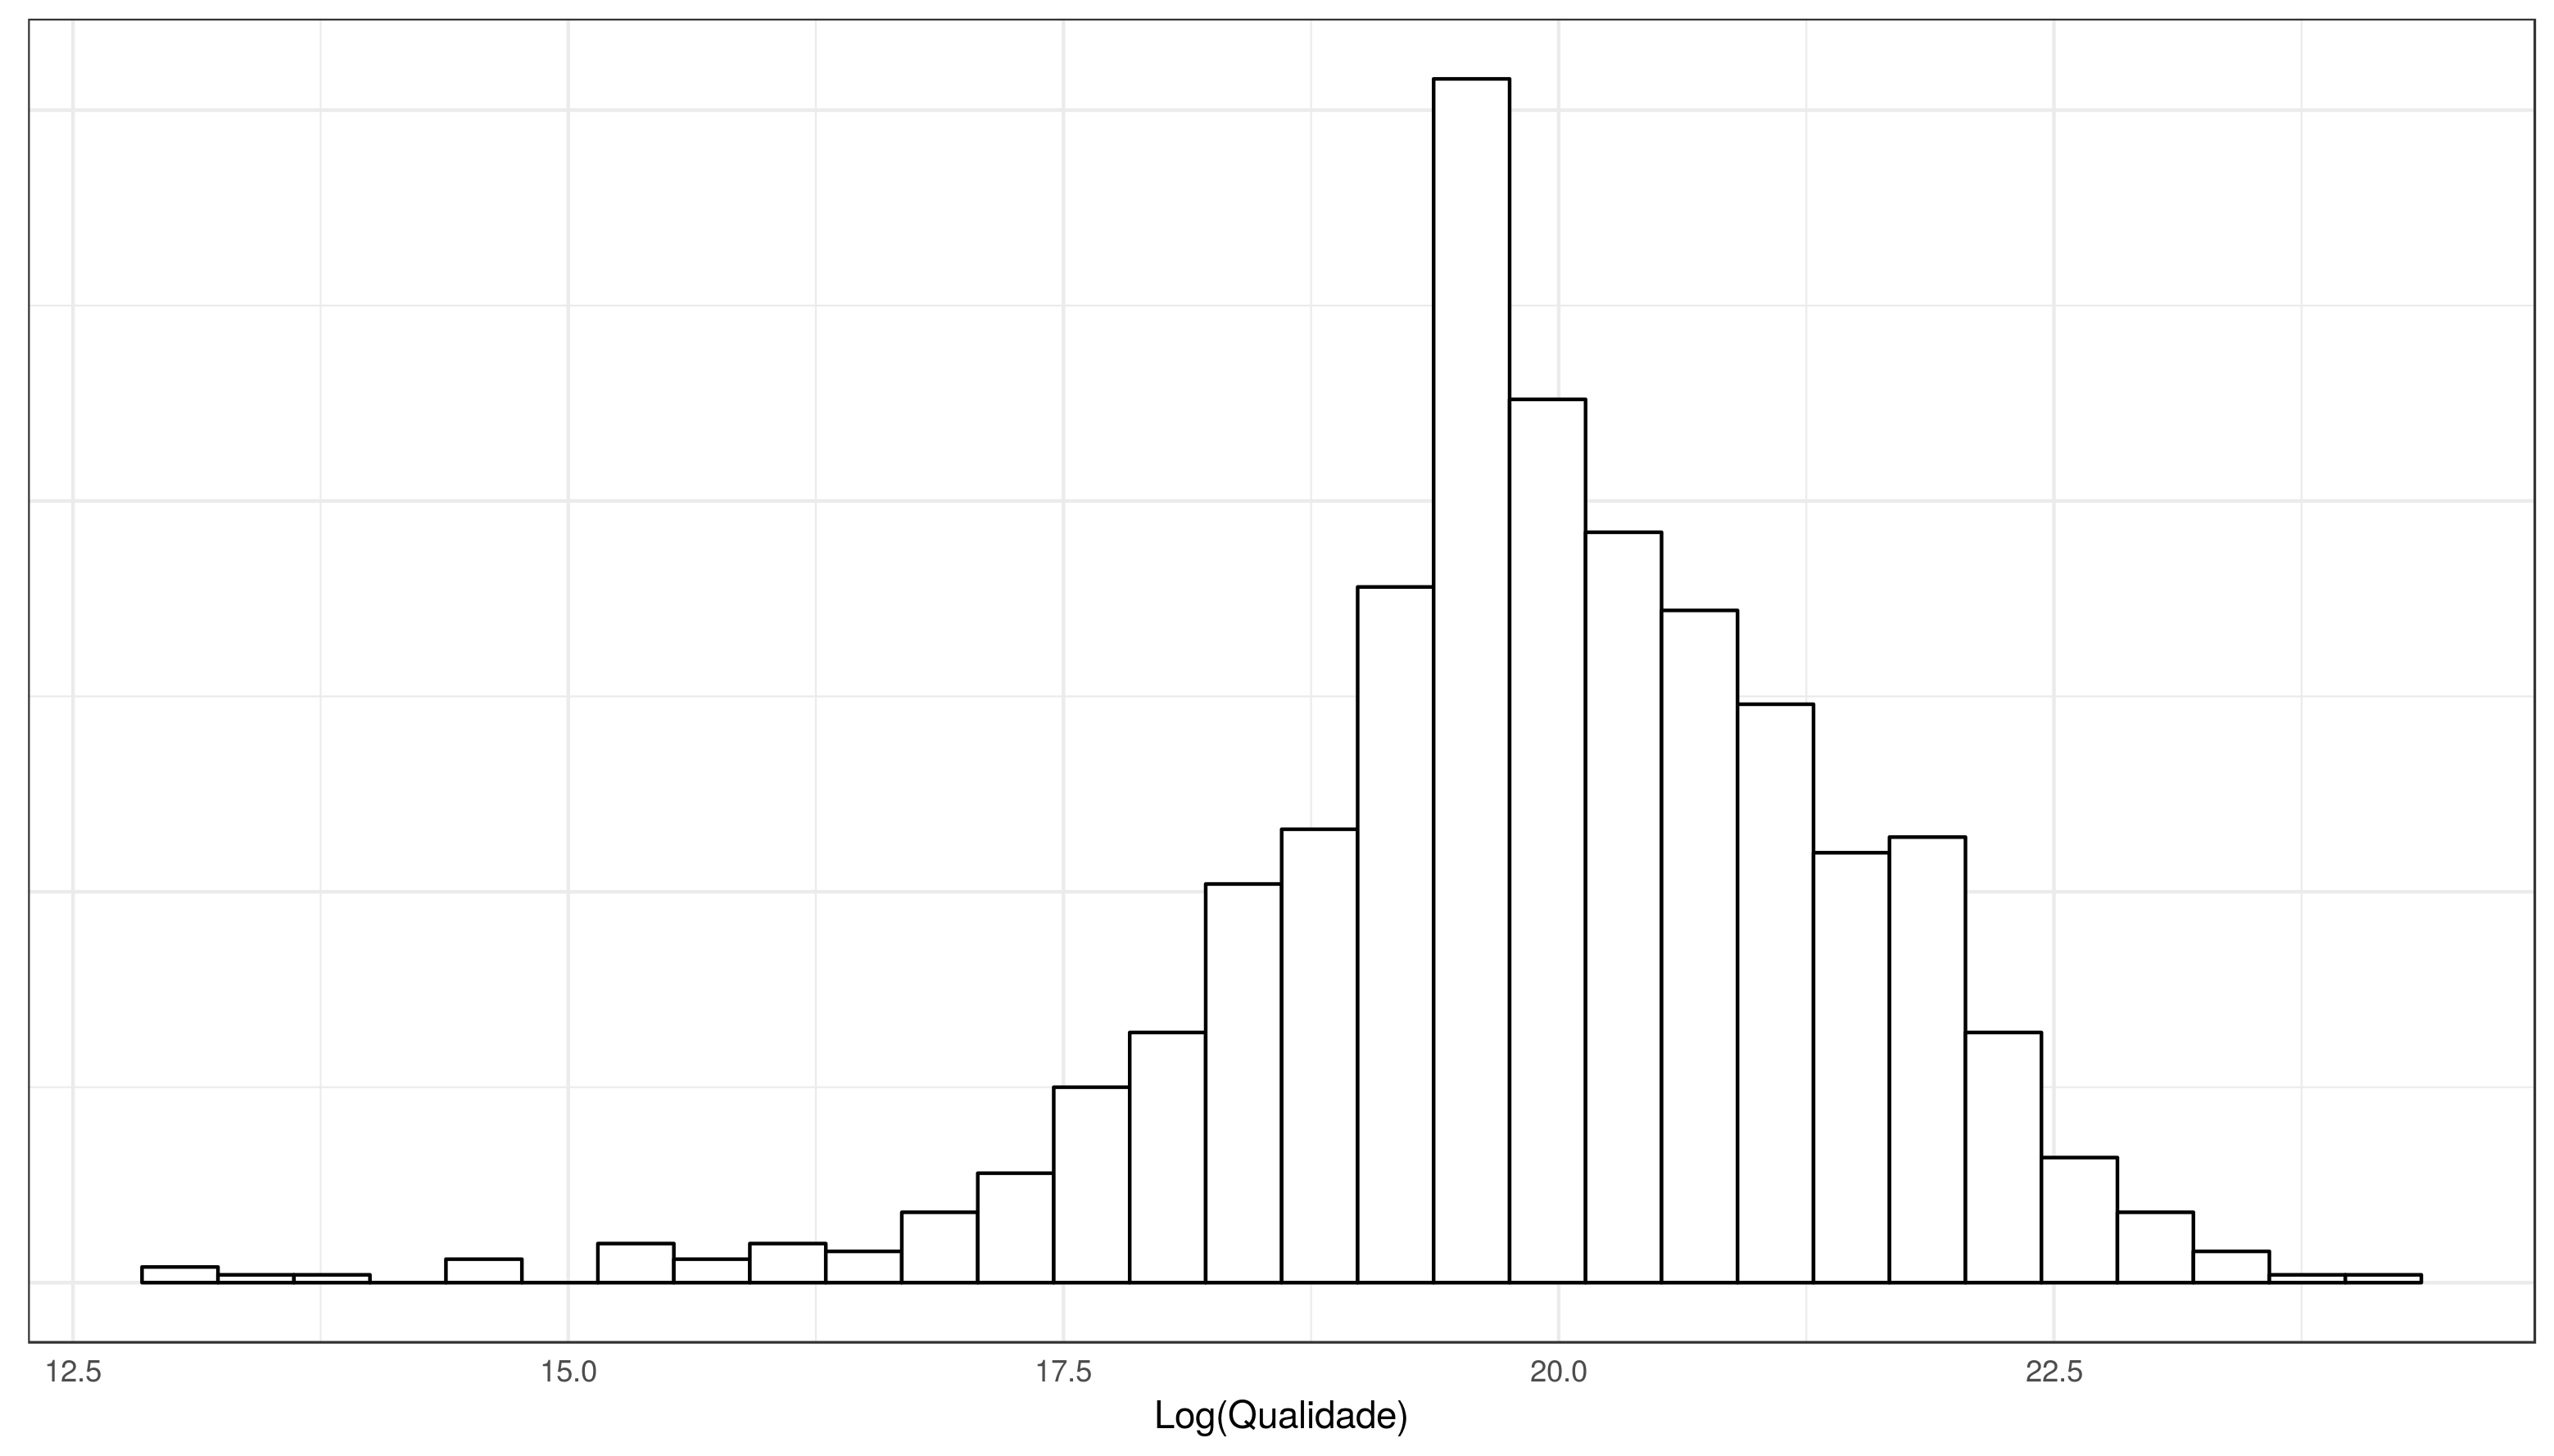
\includegraphics[width=\textwidth]{imgs/histograma_log.png}
				\caption{Histograma da Qualidade}
			\end{minipage}
			\hfill
			\begin{minipage}[b]{0.4\textwidth}
				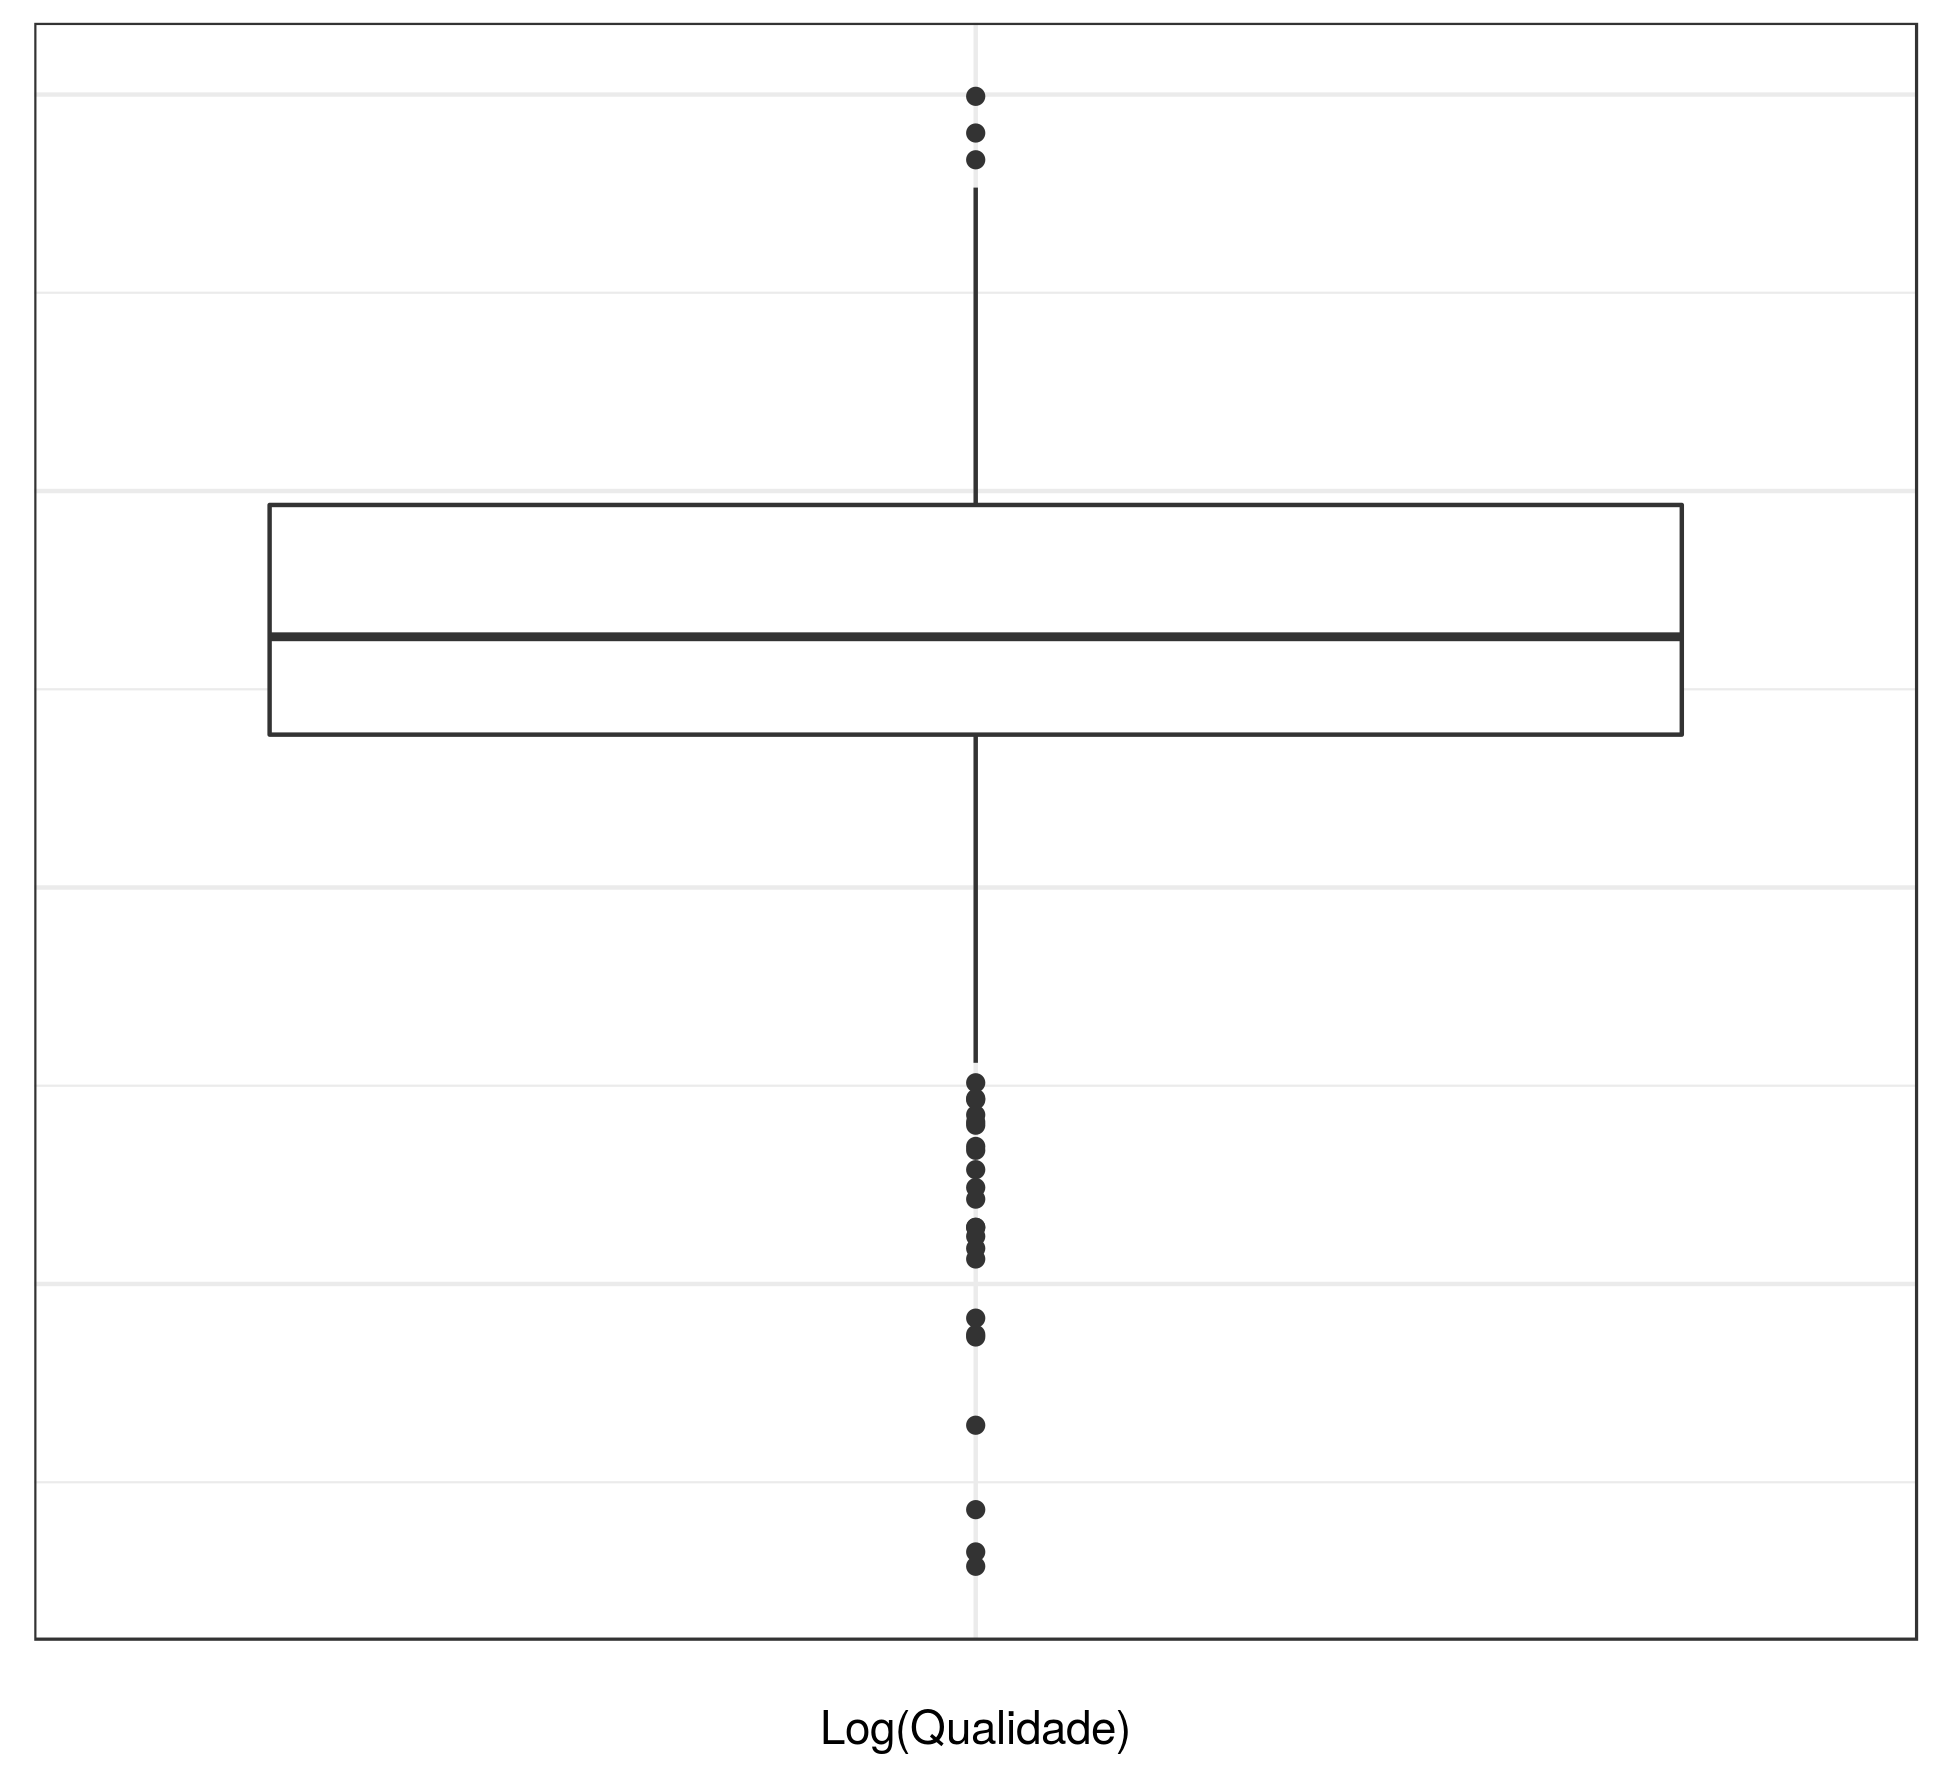
\includegraphics[width=\textwidth]{imgs/boxplot_log.png}
				\caption{Boxplot da Qualidade}
			\end{minipage}
		\end{figure}
		
		Essa é uma forma de talvez balancear melhor a amostragem dos dados da classe dominante.
		
		Assim fazemos exatamente como em $briSelect++$ e $briSelect--$ substituindo $q_k$ por $\frac{1}{q_k}$
		
	\section{Testes e Resultados}
	Os testes foram feitos utilizando os 5 métodos descritos, alem de 2 testes de referência, com todas as amostras da classe dominante e com um \textit{undersampling} aleatório dessas amostras.
	
	Foi feita uma validação cruzada com 10 \textit{folds}, para 10 arquiteturas diferentes de redes neurais \textit{multilayer perceptron} para cada uma das bases e métodos de amostragem. Então foi selecionada a arquitetura teve melhor resultado médio para cada método e base de dados.
	
	Isso foi feito para as seguintes bases :
	
	\begin{table}[H]
		\centering
		\begin{tabular}{rlrrrr}
			\hline
			& Nome & N. Pts & Pts. Dominante & Pts Minoritária & Desbalanceamento \\ 
			\hline
			& MNIST 0 vs ALL & 70000 & 63097 & 6903 & 0.11 \\ 
			& MNIST 1 vs ALL & 70000 & 62123 & 7877 & 0.13 \\ 
			& MNIST 2 vs ALL & 70000 & 63010 & 6990 & 0.11 \\ 
			& MNIST 3 vs ALL & 70000 & 62859 & 7141 & 0.11 \\ 
			& MNIST 4 vs ALL & 70000 & 63176 & 6824 & 0.11 \\ 
			& MNIST 5 vs ALL & 70000 & 63687 & 6313 & 0.10 \\ 
			& MNIST 6 vs ALL & 70000 & 63124 & 6876 & 0.11 \\ 
			& MNIST 7 vs ALL & 70000 & 62707 & 7293 & 0.12 \\ 
			& MNIST 8 vs ALL & 70000 & 63175 & 6825 & 0.11 \\ 
			& MNIST 9 vs ALL & 70000 & 63042 & 6958 & 0.11 \\ 
			& Poker Data & 1025010 & 1017261 & 7749 & 0.01 \\ 
			& Skin Data & 245057 & 194198 & 50859 & 0.26 \\ 
			\hline
		\end{tabular}
	\end{table}
	
	Assim foram obtidos os seguintes resultados em relação a AUC da média dos dados de testes.
	
	\begin{table}[H]
		\centering
		\tiny
		\begin{tabular}{rlrrrrrrr}
			\hline
			Dataset & Baseline & Undersampling & $briSelect$ & $briSelect++$ & $briSelecLog++$ & $briSelecLog--$& $briSelectLog--$ \\ 
			\hline
			0 vs ALL & 0.99 & 0.99 & 0.98 & 0.99 & 0.99 & 0.99 & 0.99 \\ 
			1 vs ALL & 0.99 & 0.99 & 0.99 & 0.99 & 0.99 & 0.99 & 0.99 \\ 
			2 vs ALL & 0.99 & 0.90 & 0.85 & 0.98 & 0.99 & 0.99 & 0.98 \\ 
			3 vs ALL & 0.99 & 0.91 & 0.83 & 0.98 & 0.98 & 0.98 & 0.98 \\ 
			4 vs ALL & 0.99 & 0.97 & 0.95 & 0.99 & 0.99 & 0.99 & 0.99 \\ 
			5 vs ALL & 0.99 & 0.86 & 0.81 & 0.98 & 0.99 & 0.98 & 0.98 \\ 
			6 vs ALL & 0.99 & 0.98 & 0.95 & 0.99 & 0.99 & 0.99 & 0.99 \\ 
			7 vs ALL & 0.99 & 0.97 & 0.91 & 0.99 & 0.99 & 0.99 & 0.99 \\ 
			8 vs ALL & 0.99 & 0.86 & 0.73 & 0.98 & 0.98 & 0.98 & 0.98 \\ 
			9 vs ALL & 0.99 & 0.92 & 0.87 & 0.98 & 0.98 & 0.98 & 0.98 \\ 
			Poker Data & 0.53 & 0.53 & 0.53 & 0.53 & 0.53 & 0.53 & 0.53 \\ 
			Skin Data & 0.99 & 0.98 & 0.94 & 0.99 & 0.98 & 0.98 & 0.94 \\ 
			\hline
		\end{tabular}
	\end{table}
	
	Em relação ao tempo de treinamento temos a seguinte tabela, onde 1 representa o tempo do modelo mais demorado para essa base  :
	
	
	  	\begin{table}[H]
	  		\centering
	  		\tiny
	  		\begin{tabular}{rlrrrrrrr}
	  			\hline
	  			Dataset & Baseline & Undersampling & $briSelect$ & $briSelect++$ & $briSelecLog++$ & $briSelecLog--$& $briSelectLog--$ \\ 
  \hline
0 vs ALL & 0.75 & 0.12 & 0.18 & 0.12 & 1.00 & 0.15 & 0.12 \\ 
1 vs ALL & 1.00 & 0.81 & 0.19 & 0.18 & 0.17 & 0.19 & 0.23 \\ 
2 vs ALL & 1.00 & 0.05 & 0.05 & 0.05 & 0.05 & 0.05 & 0.05 \\ 
3 vs ALL & 1.00 & 0.20 & 0.20 & 0.15 & 0.16 & 0.16 & 0.17 \\ 
4 vs ALL & 1.00 & 0.11 & 0.11 & 0.09 & 0.09 & 0.09 & 0.09 \\ 
5 vs ALL & 1.00 & 0.06 & 0.21 & 0.05 & 0.04 & 0.05 & 0.05 \\ 
6 vs ALL & 0.83 & 0.16 & 1.00 & 0.14 & 0.14 & 0.13 & 0.13 \\ 
7 vs ALL & 1.00 & 0.22 & 0.21 & 0.18 & 0.17 & 0.17 & 0.17 \\ 
 8 vs ALL & 1.00 & 0.05 & 0.06 & 0.05 & 0.04 & 0.05 & 0.05 \\ 
 9 vs ALL & 1.00 & 0.74 & 0.15 & 0.16 & 0.16 & 0.15 & 0.16 \\ 
Poker Data & 1.00 & 0.02 & 0.03 & 0.02 & 0.03 & 0.04 & 0.03 \\ 
Skin Data & 1.00 & 0.79 & 0.78 & 0.35 & 0.79 & 0.81 & 0.42 \\ 
  \hline
\end{tabular}
\end{table}

\section{Conclusão}
Os testes foram um tanto quanto inconclusivos. 

Foi possível observar que para as bases de dados utilizadas, o resultado das subamostragens foram extremamente similares aos resultados obtidos com todas as amostras. Nesse sentido não foi possível observar um ganho em termos de AUC.

Porém quando comparamos apenas as técnicas de \textit{undersampling}, observamos que o \textit{briSelect} claramente não é uma boa alternativa. Além disso é possível perceber que as demais técnicas que utilizam o critério de qualidade são superiores ao \textit{undersampling} aleatório. Ademais, houve uma pequena vantagem do \textit{briSelect++} e do \textit{briSelectLog++} em relação ao \textit{$briSelect--$} e o \textit{$briSelectLog--$} .

Em relação ao tempo de treinamento, quase que de forma constante, os métodos de subamostragens foram mais rápidos que o \textit{baseline}.

O trabalho ainda precisa de melhorias e mais testes. Ademais, seria interessante a criação de uma nova forma de normalizar o fator de qualidade, como por exemplo a utilização de uma medida que diferenciasse pontos da superfície de decisão à pontos da periferia  da distribuição da classe. Uma outra formar de normalizar esse critério, talvez seria a utilização da qualidade de uma media geométrica dos centros como fator de normalização.


\end{document}
